\section{Firewall}
\begin{figure}[p]
\centering
\subfloat[][\emph{Screening Router}.]{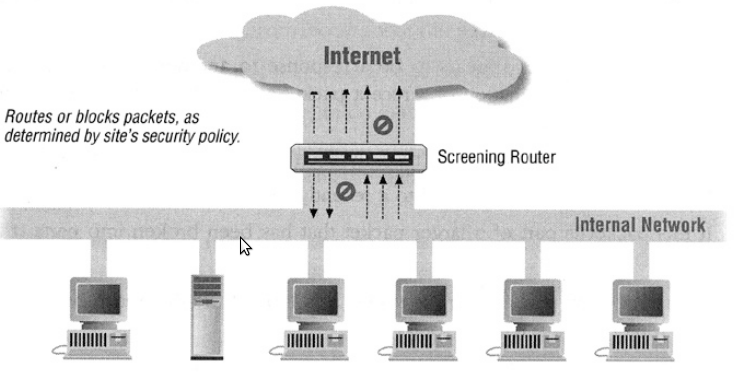
\includegraphics[scale=0.4]{images/f1.png}}\quad
\subfloat[][\emph{DualHomed Host}.]{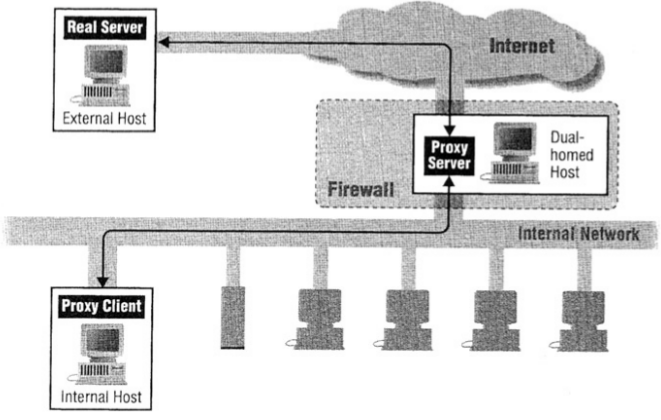
\includegraphics[scale=0.4]{images/f2.png}}\\
\subfloat[][\emph{Screened Host}.]{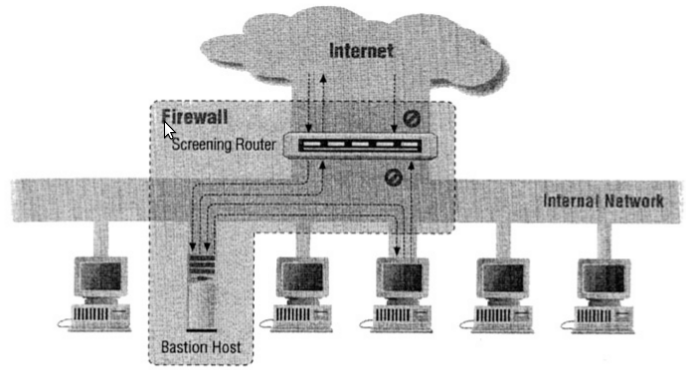
\includegraphics[scale=0.4]{images/f3.png}}\quad
\subfloat[][\emph{Screened Subnet}.]{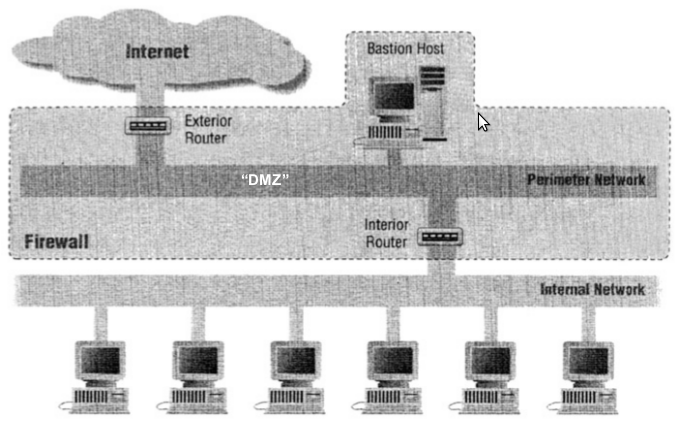
\includegraphics[scale=0.4]{images/f4.png}}\\
\caption{Esempi di Architetture Firewall.}
\end{figure}
Parliamo di \textbf{exo-structure} quando si fa riferimento agli oggetti esterni al 
sistema che stiamo considerando: ad esempio, all'interno di un sistema aziendale,
vogliamo che tale exo-structure coincida unicamente con il contatto di un unico
\textit{firewall}; anche le \textit{VPN} possono essere considerate come exo-structure(s).
I firewall sono chiamati in questo modo poiché fanno riferimento alle porte
tagliafuoco, che sono fatte per restistere agli incendi, fino ad un limite 
superiore di temperatura. In informatica questo richiama quindi il concetto del
contenimento, sottolineando il fatto che si vogliono limitare i danni il più 
possibile; essi inoltre limitano il traffico da e verso l'esterno, tramite questo
varco ben definito. Il firewall consente inoltre di:
\begin{itemize}
\item concentrare i controlli di sicurezza su di pochi punti all'interno del
	sistema, forzando a mettere in pratica le politiche di sicurezza
	precedentemente enunciate
\item possono essere utilizzate per effettuare ``auditing''
\end{itemize}
Tuttavia, tale firewall non ci può proteggere dalle minacce che provengono
dall'interno della stessa intranet aziendale: a questo scopo risulta particolarmente
inefficace se esiste una possibilità che il traffico verso l'esterno possa anche
non trasitare tramite il firewall\footnote{Ad esempio, se all'interno di questa
rete esiste un computer con accesso diretto verso l'esterno tramite un modem
seriale: in questo modo gli attaccanti potranno sfruttare le debolezze del sistema
computer, per potere poi accedere potenzialmente a tutte le informazioni dell'intranet.}.
Il firewall deve inoltre essere costantemente aggiornato, di modo da poter 
prevenire delle nuove minacce che non erano state previste precedentemente; bisogna
inoltre sottolineare come, lavorando a livello IP, non è in grado di riconoscere
le minacce relative a virus o a worm. Il firewall deve inoltre essere configurabile
solamente dall'amministratore. Sono inoltre presenti differenti tipologie di
firewall, tra le quali riconosciamo le seguenti:
\begin{itemize}
\diam Packet Filter
\diam Proxy Server
\diam Network Address Translator
\end{itemize}

\subsection{Packet Filter (o Screening Router)}
Questi meccanismi in genere vengono implementati all'interno dei routers, i quali
effettuano come compito base lo smistamento dei pacchetti, allo scopo di farli
giungere ad una prefissata destinazione: in questo caso particolare parleremo di
\textbf{screening router}.  Mentre infatti un router semplice decide vome far avvicinare 
il pacchetto alla sua destinazione, questo tipo di router prima si chiede se
quel dato pacchetto deve essere effettivamente avvicinato alla sua destinazione,
ed in caso di risposta negativa verrà cestinato.

Questo risulta inoltre possibile tramite l'analisi del pacchetto a livello
\textit{network} (siamo quindi in grado di leggerne il solo header, senza andare ad
indagare sul suo contenuto, disponibile solamente a livello applicativo). 
Considerando ciò, tale dispositivo può essere in grado di:
\begin{itemize}
\item \textit{Consentire/bloccare la comunicazione da/verso un tale IP con numero di
	porta}: lo screening router può quindi essere configurato allo scopo di
	impedire un possibile attacco che proviene da un determinato IP, oppure
	bloccando una determinata porta.
\item In quanto si ha la possibilità di avere molti possibili collegamenti in
	entrata o in uscita, si potrebbe anche stabilire di permettere il transito
	dei pacchetti di un certo tipo, tramite una sola uscita.
\item Possibilmente devono avere anche una \textit{memoria interna}, in modo da poter
	tracciare ciò che è avvenuto nel passato.
\end{itemize}
Si possono anche bloccare i pacchetti secondo le seguenti domande:
\begin{itemize}
\diam Il pacchetto è stato ricevuto dall'esterno senza una precedente particolare
	richiesta, ovvero è un pacchetto ``spontaneo''?
\diam Il pacchetto ricevuto da un particolare host esterno, ha superato un
	particolare più di un certo numero di pacchetti per unità di tempo?
\diam Si possono inoltre configurare degli stati, in modo da definire delle
	particolari politiche di sicurezza da attuare, in base ai quali effettuare
	o meno l'accettazione, ad esempio se si sono ricevuti tanti pacchetti con 
	stesso contenuto del body.
\end{itemize}
Come vantaggio dall'utilizzo di questi dispositivi, si potrebbe avere che tramite
uno solo di questi dispositivi, che tra l'altro sono efficienti e facilmente
reperibili (\textit{COTS}), si potrebbe controllare un'intera intranet; tuttavia possono essere
non banali da configurare, possono ridurre le prestazioni nella connessione di 
rete e sono ``ignoranti'' delle possoibili politiche che sono desumibili a 
livello applicativo, e quindi non riconducibili all'header IP. 

\subsection{Proxy Server}
Il termine \textit{proxy} significa ``delega'', ovvero che si concede a qualcuno
di fare certe operazioni in vece di un altro: questi strumenti sono quindi
utilizzati in modo da permettere al client di interfacciarsi con il proxy
come se questo fosse il server, ed inoltre il proxy si comporterà con il server
come se questo fosse il client. Questo è inoltre un servizio applicativo del 
server, è non è unicamente un packet filter.

Inizialmente questi dispositivi avevano solamente degli scopi di caching, o
servivano per consentire agli utenti l'accesso solamente a determinati 
contenuti: inoltre il proxy viene contattato unicamente se la comunicazione
necessita di una comunicazione verso l'esterno, e pertanto non verrà mai
contattato per le comunicazioni dell'intranet. 

In genere si utilizzano un \textbf{proxy client} all'interno dell'intranet, ed un
\textbf{proxy server} utilizzato anche come firewall, che svolge la funzione di
``dual-homed host'': questo in genere è situato esternamente alla rete locale
aziendale.

Anche in questo caso è opportuno evidenziare i suoi vantaggi con gli possibili
svantaggi: tramite questo meccanismo è possibile autentificare gli utenti che
utilizzano il servizio (possiamo quindi condcedere o meno il servizio al cliente,
ed inoltre è possibile effettuare il logging del servizio), è possibile 
filtrare i pacchetti in base al loro contenuto applicativo ed effettuare caching.
Gli svantaggi sono costituiti dal fatto che è necessario disporre di un 
proxy server, che ogni client (fungendo in quel momento da proxy client) deve
essere in grado di contattare. 

\subsection{Network Address Translator}
Una volta i NAT servivano unicamente per limitare il numero disponibile di 
indirizzi IP ($2^{32}$), allo scopo di non associare indirizzi IP all'infinito, 
senza rilasciarli quando questi non dovessero più essere utilizzati: lo scopo 
principale dei NAT è quindi quello di associare ad ognuno dei calcolatori 
all'interno della rete locale, un unico indirizzo IP che si collega ad Internet
\footnote{Altro scopo per i Router con NAT è quello di associare ad ogni
calcolatore un differente servizio di pacchetti, effettuando quindi un port-mapping
dei servizi forniti in entrata: se non fosse possibile effettuare il port-mapping,
non saremmo in grado di gestire i ``pacchetti spontanei''. Tale meccanismo si
rivela inoltre necessario per fornire servizi verso l'esterno.}. 
Questo  meccanismo può quindi essere quindi implementato all'interno di uno 
stateful router. 

Questa tecnologia ha vantaggi enormi: se i pacchetti spontanei in entrata non
sono esplicitamente ammessi, vengono rifiutati: in questo modo non si rischia
nemmeno che un potenziale attaccante possa conoscere come è strutturata la mia
rete locale. Questo NAT, in quanto comporta la riscrittura degli indirizzi del
mittente dei pacchetti, potrebbe causare dei problemi con pacchetti crittografati,
che contengono come informazione di cifratura l'indirizzo IP: inoltre in quanto
gli indirizzi IP assegnati all'interno della rete locale spesso sono dinamici,
ci potrebbero essere dei problemi con il tracciamento delle informazioni (logging).

\subsection{Architetture Firewall}
Una volta descritti i componenti possibili che possono creare un firewall, 
possiamo descrivere alcune possibili architetture:
\begin{description}
\item[Screening Router] questa è l'archiettura più semplice; include unicamente
	lo screening router che viene messo al posto di un router, ovvero sul
	limitare tra una rete interna ed una esterna: quest'ultima potrebbe
	anche non essere necessariamente Internet, ma benissimo un'altra 
	intranet.
\item[DualHomed Host] in questo caso invece si mette (es.) un Proxy Server al posto di
	un router, che quindi viene rimpiazzato da un altro host.
\item[Screened Host] assieme ad uno Screening Router, si aggiunge un \textbf{Bastion
	host}, ovvero un host fortificato dove vivono tutti i servizi che sono
	accessibili tramite l'esterno, estremamente sicuro ed aggiornato sulle
	minacce possibili; possono essere inoltre specificate ulteriori
	politiche di gestione del traffico, ad esempio si può decidere di far 
	passare tutto il flusso di informazioni in ingresso ed in uscita tramite
	il \textit{bastion host}, od oppure si può decidere che una parte del traffico 
	in uscita od in entrata, può passare tramite lo screening router, senza
	il ricorso del \textit{bastion host} intermedio.
\item[Screened Subnet] si sposta il \textit{bastion host} all'esterno dalla rete
	interna, mettendolo in una rete intermedia tra rete locale ed esterna
	chiamata \textbf{DMZ} (ovvero ``zona demilitarizzata''), che è quindi
	delimitata da un \textit{interior router} e da un \textit{exterior router}: il 
	primo può essere configurato in modo da far transitare il traffico in
	uscita solamente verso il \textit{bastion host}, il quale successivamente
	provvederà ad attuare le politiche di packet filtring appropriate,
	mentre il secondo può essere configurato in modo da far transitare 
	tutto il traffico in entrata verso lo stesso \textit{bastion host}. In questo 
	modo lo hacker deve superare due barriere minando entrambi i router.
\end{description}
